\chapter{静电场：场与高斯定理}\label{ch:b1:electrostatics-gauss}

用毛衣摩擦气球，气球便会粘在墙上；用梳子梳干燥的头发，
梳子会使一细股水流弯曲。二者背后是静止电荷之间的
作用力，即库仑定律——与引力一样，是平方反比律，
但两个质子之间的作用力强 $10^{36}$ 倍，且电荷有两种
符号，因此物质在极高的精度上呈电中性，而
其残余效应即我们所说的化学、材料乃至闪电。
本章建立使该定律便于处理的概念——\omterm{def:b1:electrostatics-gauss:field}{电场}，
说明如何由对称性读出场，并推导出
一条可在三行之内算出对称分布场的定理：
\omterm{thm:b1:electrostatics-gauss:gauss}{高斯定理}。其引力对应物
将在末尾顺带得到。

\begin{omfigure}
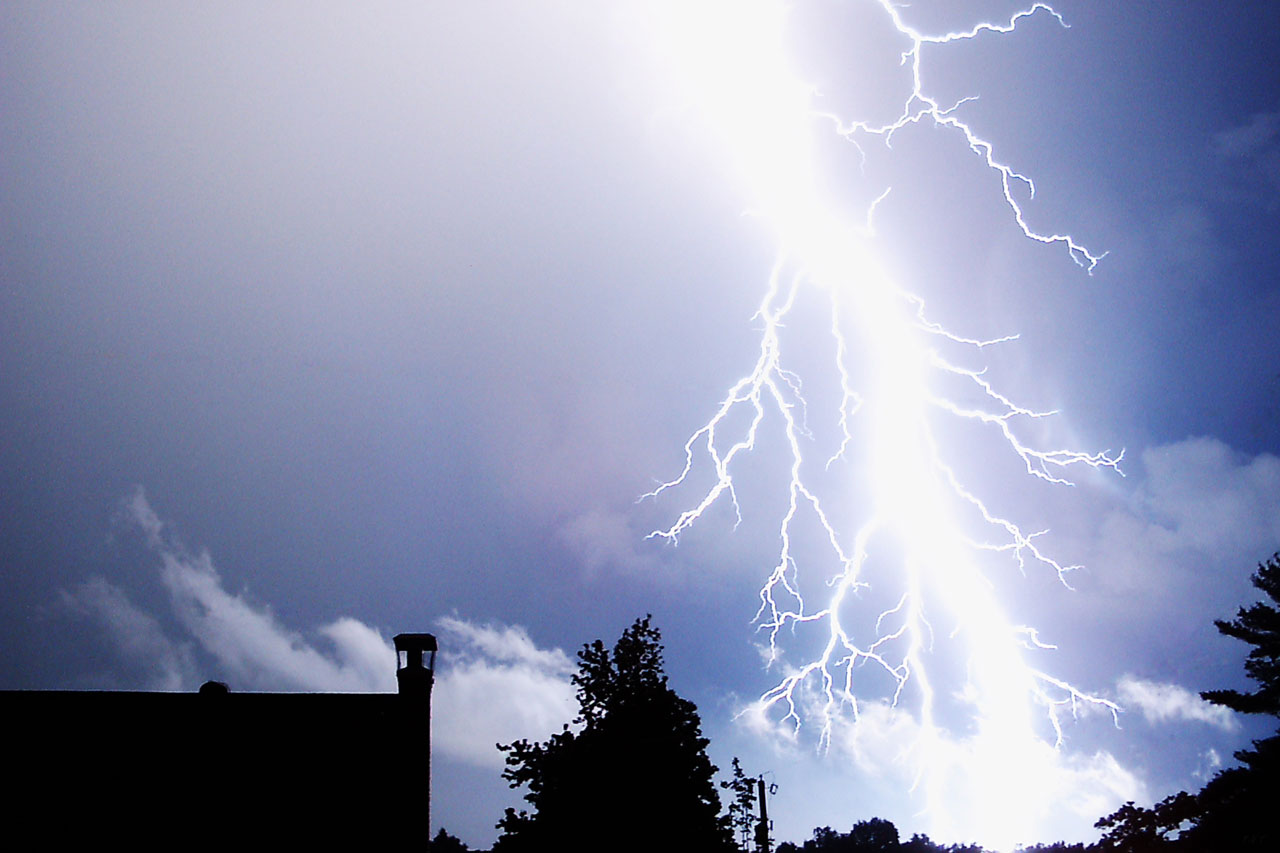
\includegraphics[width=0.50\linewidth]{images/book3/lightning-strike.jpg}

{\small 云对地闪电：数次、每次电流达一百千安的放电，可将数十库仑的电荷输送至地面——即周末问题中的带电地球。}
\end{omfigure}

\section{电荷与库仑定律}

\begin{definition}[电荷]\label{def:b1:electrostatics-gauss:charge}
\index{电荷}\index{元电荷}\index{电荷密度}
\emph{电荷} $q$（单位为库仑，\unit{C}）是物质的一种属性，
有正负两种符号；它是守恒的（孤立系统的总电荷
永不改变），并且量子化，以\emph{元电荷}为单位
$e = \qty{1.602e-19}{C}$（质子为 $+e$，电子为 $-e$）。宏观分布
可用\emph{电荷密度}描述：线电荷密度 $\lambda$
（\unit{C/m}），面电荷密度 $\sigma$（\unit{C/m^2}）或体电荷密度 $\rho$
（\unit{C/m^3}），于是微元所带电荷 $\dd q = \lambda\,\dd l$，
$\sigma\,\dd S$ 或 $\rho\,\dd\tau$。
\end{definition}

\begin{theorem}[库仑定律]\label{thm:b1:electrostatics-gauss:coulomb}
\index{库仑定律}\index{真空介电常数}
真空中静止的两个点电荷 $q_1$（位于 $M_1$）与 $q_2$（位于 $M_2$）
之间相互作用的力为
\[
\vect F_{1 \to 2} = \frac{q_1q_2}{4\pi\varepsilon_0\,r^2}\,\vect e_{12} = -\vect F_{2 \to 1},
\qquad r = M_1M_2,\quad \vect e_{12} = \frac{\vect{M_1M_2}}{r},
\]
同号电荷相斥，异号电荷相吸，其中
\emph{\omterm{thm:b1:electrostatics-gauss:coulomb}{真空介电常数}} $\varepsilon_0 = \qty{8.854e-12}{F/m}$，即
$1/4\pi\varepsilon_0 = \qty{8.99e9}{N.m^2/C^2}$。多个电荷的作用力满足
叠加原理。
\end{theorem}
\admitted

\begin{example}[有多强]\label{ex:b1:electrostatics-gauss:strong}
相距 \qty{1}{fm} 的两个质子相互排斥，斥力为 $8.99 \times 10^9 \times (1.6 \times
10^{-19})^2/10^{-30} = \qty{230}{N}$——约为一个孩子的重量，作用于两个
质量为 $10^{-27}$~kg 的粒子之间；它们之间的\omterm{def:b1:central-forces:gravitation}{万有引力}
仅为其 $10^{36}$ 分之一。两克电子置于房间一端，
等量的质子置于另一端，二者将以 $10^{25}$~N 的力相互吸引。
物质呈电中性，是因为别无选择：任何失衡都会被
任何结构都无法抗拒的力所纠正。
\end{example}

\section{电场}

\begin{definition}[静电场]\label{def:b1:electrostatics-gauss:field}
\index{电场}\index{场线}
静止电荷的分布在空间每一点 $M$ 处
产生一个\emph{电场} $\vect E(M)$，它由作用于
试探电荷 $q$（位于 $M$ 处）上的力定义：$\vect F = q\vect E(M)$（\unit{V/m} $=$
\unit{N/C}）。点电荷 $q_1$（位于 $O$ 处）产生的场为
\[
\vect E(M) = \frac{q_1}{4\pi\varepsilon_0 r^2}\,\vect e_r , \qquad r = OM ,
\]
沿径向，$q_1 > 0$ 时向外；分布产生的场为其各微元场的
矢量和。\emph{场线}是一条曲线，它在每一点都与
$\vect E$ 相切，并沿其方向取向。
\end{definition}

\begin{proposition}[读懂场线图]\label{prop:b1:electrostatics-gauss:lines}
\omterm{def:b1:electrostatics-gauss:field}{场线}从正电荷出发，止于负电荷（或止于
无穷远）；\omterm{def:b1:electrostatics-gauss:field}{场线}永不相交（场是单值的），并且
在场强较大处更为密集。若存在两个电荷，
从每个电荷发出的\omterm{def:b1:electrostatics-gauss:field}{场线}数与其电荷量成正比。
\end{proposition}

\begin{omfigure}
\begin{tikzpicture}[font=\small, x=1cm, y=1cm, >=Stealth]
  % dipole: arcs through (-1,0) and (1,0), centre (0,c)
  \begin{scope}[scale=1.4]
    \foreach \c in {0.1, 0.55, 1.6} {
      \draw[omDef, thick, postaction={decorate, decoration={markings, mark=at position 0.5 with {\arrow{>}}}}]
        let \n1 = {sqrt(1+\c*\c)} in
        (-1,0) arc[start angle={180+atan2(\c,1)}, end angle={360-atan2(\c,1)}, radius=\n1 cm];
      \draw[omDef, thick, postaction={decorate, decoration={markings, mark=at position 0.5 with {\arrow{>}}}}]
        let \n1 = {sqrt(1+\c*\c)} in
        (-1,0) arc[start angle={180-atan2(\c,1)}, end angle={atan2(\c,1)}, radius=\n1 cm];
    }
    \draw[omDef, thick, postaction={decorate, decoration={markings, mark=at position 0.5 with {\arrow{>}}}}] (-1,0) -- (1,0);
    \draw[omDef, thick, postaction={decorate, decoration={markings, mark=at position 0.6 with {\arrow{>}}}}] (-2.6,0) -- (-1,0);
    \draw[omDef, thick, postaction={decorate, decoration={markings, mark=at position 0.4 with {\arrow{>}}}}] (1,0) -- (2.6,0);
    \fill[omThm] (-1,0) circle (3pt) node[below left] {$+q$};
    \fill[omDef] (1,0) circle (3pt) node[below right] {$-q$};
  \end{scope}
  % two like charges
  \begin{scope}[xshift=7.9cm, fl/.style={omThm, thick, postaction={decorate, decoration={markings, mark=at position 0.55 with {\arrow{>}}}}}]
    \foreach \s in {1,-1} {
      % left charge at (-1,0), right charge at (1,0); \s mirrors up/down
      \draw[fl] (-1,0) -- (-3.4,0);
      \draw[fl] (1,0) -- (3.4,0);
      \draw[fl] (-1,0) .. controls (-2.2,{1.2*\s}) .. (-3.2,{2.0*\s});
      \draw[fl] (1,0) .. controls (2.2,{1.2*\s}) .. (3.2,{2.0*\s});
      \draw[fl] (-1,0) .. controls (-1.1,{1.3*\s}) .. (-1.6,{2.9*\s});
      \draw[fl] (1,0) .. controls (1.1,{1.3*\s}) .. (1.6,{2.9*\s});
      \draw[fl] (-1,0) .. controls (-0.2,{0.7*\s}) and (-0.1,{1.6*\s}) .. (-0.3,{2.9*\s});
      \draw[fl] (1,0) .. controls (0.2,{0.7*\s}) and (0.1,{1.6*\s}) .. (0.3,{2.9*\s});
    }
    \draw[fl] (-1,0) -- (-0.08,0);
    \draw[fl] (1,0) -- (0.08,0);
    \fill[omThm] (-1,0) circle (3pt) node[below left] {$+q$};
    \fill[omThm] (1,0) circle (3pt) node[below right] {$+q$};
    \fill (0,0) circle (1.2pt) node[below, font=\footnotesize, yshift=-2pt] {$\vect E = \vect 0$};
  \end{scope}
\end{tikzpicture}

{\small 两个异号电荷（左）与两个等量正电荷（右）的\omterm{def:b1:electrostatics-gauss:field}{场线}。
\omterm{def:b1:electrostatics-gauss:field}{场线}始于 $+$，止于 $-$ 或无穷远；在右图中，两个正电荷相互排斥，
场在中点处为零，
该点处无\omterm{def:b1:electrostatics-gauss:field}{场线}经过。}
\end{omfigure}

\begin{example}[直接求和：圆环与线段]\label{ex:b1:electrostatics-gauss:ring}
设半径为 $R$ 的圆环均匀带电 $Q$，在其轴线上距圆心
$z$ 处，每个电荷元 $\dd q$ 的场贡献为 $\dd q/4\pi\varepsilon_0(R^2 +
z^2)$，方向沿其与 $M$ 的连线；垂直于轴线的分量两两相消，
轴向分量则相加，每项乘以因子
$z/\sqrt{R^2 + z^2}$，结果为：
\[
E_z = \frac{Qz}{4\pi\varepsilon_0(R^2 + z^2)^{3/2}} ,
\]
在中心处为零，在 $z = R/\sqrt2$ 处最大，远处
为 $Q/4\pi\varepsilon_0z^2$。均匀带电圆盘可看作一叠圆环（见\cref{pb:b1:electrostatics-gauss:1}）。
只要几何条件允许写出积分，直接求和即可；
本章其余部分的目的正是避免这种做法。
\end{example}

\section{对称性与不变性}

\begin{proposition}[对称性原理]\label{prop:b1:electrostatics-gauss:symmetry}
\index{场的对称性}\index{对称面}\index{反对称面}
场具有其源的对称性。若平面 $\Pi$ 是电荷分布的
\emph{\omterm{prop:b1:electrostatics-gauss:symmetry}{对称面}}（分布关于它的镜像即其自身），则 $\Pi$ 上每点的场
都\emph{位于} $\Pi$ 内；
若 $\Pi$ 是\emph{\omterm{prop:b1:electrostatics-gauss:symmetry}{反对称面}}（镜像分布是各电荷全部反号后的分布），
则 $\Pi$ 上各点处的场\emph{垂直于} $\Pi$。
若分布在平移或转动下不变，
则场也如此，
其分量不依赖于相应的坐标。
\end{proposition}

\begin{proof}
$\vect E$ 是若干项 $\dd q\,\vect e/4\pi\varepsilon_0r^2$ 之和；和的镜像
等于各项镜像之和，而分布场的镜像
即镜像分布的场（一个由位置与电荷构成的矢量
按与位置相同的方式变换）。在
\omterm{prop:b1:electrostatics-gauss:symmetry}{对称面}上，场与其镜像相同，因此位于该面内；
在\omterm{prop:b1:electrostatics-gauss:symmetry}{反对称面}上，场与其镜像互为相反数，
因此与该面垂直。不变性的论证与此相同，只需把镜像换成
平移或转动。
\end{proof}

\begin{method}[计算前先确定场的形状]\label{meth:b1:electrostatics-gauss:symmetry}
对所求场的点 $M$：(1) 列出包含 $M$ 的
源的\omterm{prop:b1:electrostatics-gauss:symmetry}{对称面}——场位于它们的
交线上；两个这样的\omterm{prop:b1:electrostatics-gauss:symmetry}{对称面}即可确定方向。(2) 列出
不变性——它们给出 $\vect E$ 依赖于哪些坐标。因此
均匀带电的无限长导线在\omterm{def:b1:point-kinematics:cylindrical}{柱坐标}中给出 $\vect E = E(r)\,\vect e_r$，
球体在\omterm{def:b1:point-kinematics:spherical}{球坐标}中给出 $\vect E = E(r)\,\vect e_r$，
无限大平面给出 $\vect E = E(z)\,\vect e_z$，且 $E(-z) = -E(z)$。
此后方可进行计算。
\end{method}

\begin{omfigure}
\begin{tikzpicture}[font=\small, x=1cm, y=1cm, >=Stealth]
  % sphere
  \begin{scope}
    \draw[omDef, fill=omDef!15] (0,0) circle (0.9);
    \draw[dashed] (0,0) circle (1.8);
    \foreach \a in {0,45,...,315} \draw[omThm, thick, ->] (\a:1.8) -- ++(\a:0.6);
    \node[font=\footnotesize] at (0,-2.75) {$\vect E = E(r)\,\vect e_r$};
    \node[font=\footnotesize, omDef] at (0,0) {$Q$};
  \end{scope}
  % cylinder / wire
  \begin{scope}[xshift=5.2cm]
    \draw[omDef, very thick] (0,-2.2) -- (0,2.2) node[above, font=\footnotesize] {$\lambda$};
    \draw[dashed] (-1.1,-1.6) rectangle (1.1,1.6);
    \draw[dashed] (0,1.6) ellipse (1.1 and 0.28);
    \draw[dashed] (0,-1.6) ellipse (1.1 and 0.28);
    \foreach \y in {-1.0,-0.3,0.4,1.1} {\draw[omThm, thick, ->] (1.1,\y) -- ++(0.6,0); \draw[omThm, thick, ->] (-1.1,\y) -- ++(-0.6,0);}
    \node[font=\footnotesize] at (0,-2.75) {$\vect E = E(r)\,\vect e_r$（柱坐标）};
  \end{scope}
  % plane
  \begin{scope}[xshift=10.4cm]
    \draw[omDef, fill=omDef!25] (-1.8,-0.25) -- (1.8,-0.25) -- (2.2,0.25) -- (-1.4,0.25) -- cycle;
    \node[omDef, font=\footnotesize] at (1.9,-0.45) {$\sigma$};
    \draw[dashed] (-0.5,-1.4) rectangle (0.5,1.4);
    \foreach \x in {-1.2,0,1.2} {\draw[omThm, thick, ->] (\x,0.35) -- ++(0,0.9); \draw[omThm, thick, ->] (\x,-0.35) -- ++(0,-0.9);}
    \node[font=\footnotesize] at (0,-2.75) {$\vect E = E(z)\,\vect e_z$，关于 $z$ 为奇};
  \end{scope}
\end{tikzpicture}

{\small 本章的三种对称分布，以及与之相适应的
高斯面（虚线）：同心球面、同轴圆柱面，
以及跨越平面的扁盒。在每个高斯面上，场
要么法向且大小均匀，要么切向。}
\end{omfigure}

\section{通量与高斯定理}

\begin{definition}[场的通量]\label{def:b1:electrostatics-gauss:flux}
\index{电场的通量}
将曲面 $S$ 分割为许多面积为 $\dd S$ 的小面元，每个面元上取单位法向量 $\vect n$
（对闭合曲面取外法向）。$\vect E$ 穿过 $S$ 的
\emph{通量}是下述和式：
\[
\Phi = \sum \vect E\cdot\vect n\,\dd S = \sum E_n\,\dd S \qquad (\unit{V.m}):
\]
场的法向分量按面积加权——即穿过 $S$ 的“\omterm{def:b1:electrostatics-gauss:field}{场线}
数”，计正的穿过方向为沿
$\vect n$.
\end{definition}

\begin{theorem}[高斯定理]\label{thm:b1:electrostatics-gauss:gauss}
\index{高斯定理}
静\omterm{def:b1:electrostatics-gauss:field}{电场}穿过任一闭合曲面 $S$ 的\omterm{def:b1:electrostatics-gauss:flux}{通量}，
等于 $S$ 所包围的总电荷除以 $\varepsilon_0$：
\[
\Phi_{\text{外}} = \frac{Q_{\text{内}}}{\varepsilon_0} .
\]
$S$ 之外的电荷对\omterm{def:b1:electrostatics-gauss:flux}{通量}没有贡献（其\omterm{def:b1:electrostatics-gauss:field}{场线}
进入后又穿出）。
\end{theorem}

\begin{proof}
对位于球心处的点电荷 $q$，球面半径为 $r$：
$\vect E$ 沿径向，在球面上处处大小为 $q/4\pi\varepsilon_0r^2$，
于是 $\Phi = E \times 4\pi r^2 = q/\varepsilon_0$——与 $r$ 无关，
这是因为场按 $1/r^2$ 衰减，恰与面积的增长相抵。
同样的结论对包围 $q$ 的任一闭合曲面成立（通过一个面元的\omterm{def:b1:electrostatics-gauss:flux}{通量}
只取决于该面元从 $q$ 处所张的立体角），
外部电荷的\omterm{def:b1:electrostatics-gauss:flux}{通量}为零（它对每个立体角都张了两次，
符号相反），以及若干电荷的\omterm{def:b1:electrostatics-gauss:flux}{通量}可以相加，这些结论
在本阶段不加证明地承认；完整证明见本科二年级分册。
\end{proof}

\begin{method}[使用高斯定理]\label{meth:b1:electrostatics-gauss:gauss}
(1) 由对称性写出 $\vect E$ 的形式（方向，以及它所依赖的
变量）。(2) 选取一个闭合的\emph{高斯面}，
使其过点 $M$，且 $\vect E$ 在其上处处要么与曲面垂直、大小都为 $E(M)$，
要么与曲面相切；此时\omterm{def:b1:electrostatics-gauss:flux}{通量}等于 $E(M)$ 乘以法向部分的
面积。(3) 数出内部的电荷。(4) 由此解出
$E(M)$。该方法适用于球面、无限长圆柱面与无限大平面，
——其他情形在无进一步工具时均不适用。
\end{method}

\begin{proposition}[三种经典场]\label{prop:b1:electrostatics-gauss:three}
\index{带电球体的场}\index{带电导线的场}\index{带电平面的场}
\begin{enumerate}
  \item 半径为 $R$ 的球体，电荷 $Q$ 均匀分布于其
        体积内：外部 $E(r) = \dfrac{Q}{4\pi\varepsilon_0r^2}$（$r > R$）——
        如同全部电荷都集中于球心——而内部 $E(r) =
        \dfrac{Qr}{4\pi\varepsilon_0R^3}$，从零开始线性增长；
        在 $r = R$ 处连续。若电荷只分布于表面，
        则内部场为零。
  \item 线\omterm{def:b1:electrostatics-gauss:charge}{电荷密度}为 $\lambda$ 的无限长导线：$E(r) =
        \dfrac{\lambda}{2\pi\varepsilon_0 r}$，沿径向。
  \item 面\omterm{def:b1:electrostatics-gauss:charge}{电荷密度}为 $\sigma$ 的无限大平面：$E = \dfrac{\sigma}{2\varepsilon_0}$
        位于平面两侧，垂直于平面，
        当 $\sigma > 0$ 时指向远离平面的方向，\emph{与距离无关}。穿过平面时，
        法向分量跃变 $\sigma/\varepsilon_0$。
\end{enumerate}
\end{proposition}

\begin{proof}
(1) 半径为 $r$ 的球面：\omterm{def:b1:electrostatics-gauss:flux}{通量}为 $4\pi r^2E(r)$；内部电荷
为 $Q$（$r > R$ 时），$Q(r/R)^3$（$r < R$ 时）。(2) 半径为 $r$、长为 $h$ 的圆柱面：
侧面\omterm{def:b1:electrostatics-gauss:flux}{通量}为 $2\pi rh\,E(r)$，两端面无\omterm{def:b1:electrostatics-gauss:flux}{通量}
（场与之相切）；内部电荷为 $\lambda h$。(3) 横截面积为 $S$ 的扁圆柱面，
跨在平面两侧：通过两端面的\omterm{def:b1:electrostatics-gauss:flux}{通量}为 $2SE$（场关于 $z$ 为奇函数，
两端的贡献都取正），侧面无\omterm{def:b1:electrostatics-gauss:flux}{通量}；内部电荷为
$\sigma S$。
\end{proof}

\begin{omfigure}
\begin{tikzpicture}
\begin{axis}[omaxis, axis x line=bottom, axis y line=left, width=10cm, height=5.6cm,
    xlabel={$r/R$}, ylabel={$E$（单位为 $Q/4\pi\varepsilon_0R^2$）},
    xlabel style={at={(axis description cs:0.5,-0.1)}, anchor=north},
    xmin=0, xmax=4, ymin=0, ymax=1.3, xtick={1,2,3}, ytick={0.5,1}, samples=80]
  \addplot[omDef, very thick, domain=0:1] {x} node[pos=0.85, above left, font=\footnotesize] {体积分布：$\propto r$};
  \addplot[omDef, very thick, domain=1:4] {1/x^2} node[pos=0.35, above right, font=\footnotesize] {$\propto 1/r^2$};
  \addplot[omThm, thick, dashed] coordinates {(0,0) (1,0)};
  \addplot[omThm, thick, dashed] coordinates {(1,0) (1,1)};
  \node[omThm, font=\footnotesize, anchor=west] at (axis cs:1.08,0.08) {表面分布：内部为 $0$};
\end{axis}
\end{tikzpicture}

{\small \omterm{prop:b1:electrostatics-gauss:three}{带电球体的场}随到球心距离的变化：
电荷充满体积时，内部线性增长、外部按 $1/r^2$ 衰减，
（实线）；电荷只在表面时，内部为零、外部相同
（虚线）。在外部，球体与位于其球心的点电荷
无从区分。}
\end{omfigure}

\begin{example}[两块平行板电容器]\label{ex:b1:electrostatics-gauss:twoplanes}
\index{平行板电容器!场}
两个平行平面分别带有 $+\sigma$ 和 $-\sigma$：每个平面各自产生
大小为 $\sigma/2\varepsilon_0$ 的场，正平面的场背离它，负平面的场指向它。
两平面之间，两场叠加为 $\sigma/\varepsilon_0$，方向由
$+$ 指向 $-$；两平面之外，两场相互抵消。取 $\sigma = \qty{1}{\micro C/m^2}$，$E =
10^{-6}/8.85 \times 10^{-12} = \qty{1.1e5}{V/m}$，两平面之间为该值，外部为零：
即带电电容器的场被限制在其间隙之内
（见\cref{ch:b1:potential-capacitors}）。
\end{example}

\begin{omfigure}
\begin{tikzpicture}[font=\small, x=1cm, y=1cm, >=Stealth]
  \draw[omThm, very thick] (-0.8,-2) -- (-0.8,2) node[above] {$+\sigma$};
  \draw[omDef, very thick] (0.8,-2) -- (0.8,2) node[above] {$-\sigma$};
  % field of + plane (red), of - plane (blue), resultant (black)
  \foreach \y in {-1.4,-0.7,0,0.7,1.4} {
    \draw[omThm, ->] (-0.8,\y) -- ++(0.55,0);
    \draw[omThm, ->] (-0.8,\y) -- ++(-0.55,0);
    \draw[omDef, ->] (0.8,\y) -- ++(-0.55,0);
    \draw[omDef, ->] (0.8,\y) -- ++(0.55,0);
  }
  \node[omThm, font=\footnotesize, anchor=east] at (-1.0,-2.4) {$+\sigma$ 单独存在：$\sigma/2\varepsilon_0$};
  \node[omDef, font=\footnotesize, anchor=west] at (1.0,-2.4) {$-\sigma$ 单独存在：$\sigma/2\varepsilon_0$};
  \begin{scope}[xshift=7.2cm]
    \draw[omThm, very thick] (-0.8,-2) -- (-0.8,2) node[above] {$+\sigma$};
    \draw[omDef, very thick] (0.8,-2) -- (0.8,2) node[above] {$-\sigma$};
    \foreach \y in {-1.4,-0.7,0,0.7,1.4} \draw[black, very thick, ->] (-0.75,\y) -- (0.7,\y);
    \node[font=\footnotesize] at (0,-2.4) {合场：两板之间为 $\sigma/\varepsilon_0$，外部为 $0$};
  \end{scope}
\end{tikzpicture}

{\small 两块相反带电平面的叠加。左：各平面单独产生的匀强场
（红色来自正平面，蓝色指向负平面）。
右：二者之和，$\sigma/\varepsilon_0$ 位于间隙中，其余处为零。}
\end{omfigure}

\section{引力类比}

\begin{proposition}[引力的高斯定理]\label{prop:b1:electrostatics-gauss:gravity}
\index{高斯定理!引力}\index{引力场}
牛顿定律 $\vect F = -Gm_1m_2\,\vect e_{12}/r^2$ 与库仑定律形式相同，
只需将 $q \to m$，$1/4\pi\varepsilon_0 \to -G$。
因此\omterm{prop:b1:newton-dynamics:weight}{引力场} $\vect g$（单位质量所受的力）服从相同的对称性规则，
并满足
\[
\Phi_{\text{外}}(\vect g) = -4\pi G\,M_{\text{内}} .
\]
特别地，球对称物体对外部各点的吸引，与其质量
全部集中于球心时相同；
半径为 $R$、质量为 $M$ 的均匀球体内部，场为 $g(r) = GMr/R^3$，与 $r$ 成正比。
\end{proposition}

\begin{proof}
将 $Q/\varepsilon_0$ 替换为 $-4\pi GM$，即可沿用
\cref{prop:b1:electrostatics-gauss:three}的证明；负号表示
\omterm{def:b1:electrostatics-gauss:flux}{通量}流入（引力是吸引的）。
\end{proof}

\begin{example}[地球内部]\label{ex:b1:electrostatics-gauss:earth}
对于均匀地球，$g$ 将从地表处的 \qty{9.8}{m/s^2} 线性
减小到地心处的零；若石块从穿过行星的隧道落下，
将做简谐振动，周期为 $2\pi\sqrt{R/g} =
\qty{84}{min}$——恰为掠地卫星的周期。真实地球具有
致密的地核，$g$ 在地核–地幔边界处实际上\emph{升高}到 \qty{10.7}{m/s^2}，
随后才下降（见\cref{pb:b1:electrostatics-gauss:1}）。
牛顿需要壳层定理，才能将其定律应用于行星；\omterm{thm:b1:electrostatics-gauss:gauss}{高斯
定理}一行即可给出结果。
\end{example}

\section{练习}

\begin{exercise}[$\star$]\label{exo:b1:electrostatics-gauss:1}
求两质子之间的电力与引力，
两者相距 \qty{2.0}{fm}；并求其比值。原子核为何仍能结合在一起？
\end{exercise}

\begin{exercise}[$\star$]\label{exo:b1:electrostatics-gauss:2}
求距 \qty{1.0}{m} 处、由 \qty{1.0}{\micro C} 点电荷产生的场强。地球表面
的场强为 \qty{100}{V/m}，方向竖直向下：求地球所带电荷的符号与大小，
并将地球视为半径为 \qty{6370}{km} 的球体。
\end{exercise}

\begin{exercise}[$\star$]\label{exo:b1:electrostatics-gauss:3}
两电荷 $+q$ 位于 $x = \pm a$ 处（均在 $x$ 轴上）。求 $x$ 轴上
$|x| > a$ 时的场，以及 $y$ 轴上的场；证明 $y$ 轴上 $E_y$
在 $y = a/\sqrt2$ 处取得最大值。画出原点附近的\omterm{def:b1:electrostatics-gauss:field}{场线}示意图。
\end{exercise}

\begin{exercise}[$\star$]\label{exo:b1:electrostatics-gauss:4}
电荷 $+2q$ 位于 $x = 0$ 处，$-q$ 位于 $x = a$ 处。求 $x$ 轴上
场强为零的位置？从 $+2q$ 发出的\omterm{def:b1:electrostatics-gauss:field}{场线}数与到达 $-q$ 的\omterm{def:b1:electrostatics-gauss:field}{场线}数之比为多少？
其余\omterm{def:b1:electrostatics-gauss:field}{场线}去向何方？
\end{exercise}

\begin{exercise}[$\star\star$]\label{exo:b1:electrostatics-gauss:5}
半径为 $R$ 的圆盘均匀带电，面\omterm{def:b1:electrostatics-gauss:charge}{电荷密度}为 $\sigma$。由环的结果，
在其轴线上证明 $E_z = \dfrac{\sigma}{2\varepsilon_0}\Bigl(1 - \dfrac{z}{\sqrt{z^2 +
R^2}}\Bigr)$（$z > 0$）；并检验 $z \ll R$ 与 $z \gg R$ 两种极限情形。
\end{exercise}

\begin{exercise}[$\star\star$]\label{exo:b1:electrostatics-gauss:6}
将金原子核（$Z = 79$，$R = \qty{7.0}{fm}$）视为均匀带电
球体，求其表面处、$R/2$ 处以及距中心 \qty{1}{pm} 处的场强。
并与空气的击穿场强 \qty{3e6}{V/m} 进行比较。
\end{exercise}

\begin{exercise}[$\star\star$]\label{exo:b1:electrostatics-gauss:7}
用\omterm{thm:b1:electrostatics-gauss:gauss}{高斯定理}求无限长直导线的场。某高压导体
半径为 \qty{1.0}{cm}：求线\omterm{def:b1:electrostatics-gauss:charge}{电荷密度}为多大时其表面场强
达到击穿值 \qty{3e6}{V/m}（电晕起始）。此时
求距轴线 \qty{5}{m} 处的场强。
\end{exercise}

\begin{exercise}[$\star\star$]\label{exo:b1:electrostatics-gauss:8}
两平行极板面积为 \qty{1.0}{m^2}，分别带电 $\pm\qty{1.0}{\micro C}$。
求两板间的场强；求一块极板所受的力（作用于其上的场仅来自另一块极板——
为什么？）；并求极板上的压强。
\end{exercise}

\begin{exercise}[$\star\star$]\label{exo:b1:electrostatics-gauss:9}
同轴电缆：内导体半径为 $a$、带电 $+\lambda$，外
护套半径为 $b$、带电 $-\lambda$，用\omterm{thm:b1:electrostatics-gauss:gauss}{高斯定理}求三个区域中
的场强。取 $a = \qty{0.5}{mm}$，$b = \qty{2.5}{mm}$，$\lambda = \qty{10}{nC/m}$，
求内导体表面处的场强。
\end{exercise}

\begin{exercise}[$\star\star\star$]\label{exo:b1:electrostatics-gauss:10}
厚球壳 $R_1 < r < R_2$ 的体内均匀带有电荷 $Q$，
求三个区域中的场强，并检验在 $R_1$
与 $R_2$ 处的连续性；场强在何处最大？画出 $E(r)$ 的草图。一正电荷
置于空腔内，它受到怎样的力？
\end{exercise}

\begin{exercise}[$\star\star\star$]\label{exo:b1:electrostatics-gauss:11}
\emph{地球内部的引力。}地核半径为 \qty{3480}{km}，密度
为 \qty{11000}{kg/m^3}；地幔延伸至 \qty{6370}{km}，密度为 \qty{4500}{kg/m^3}。
(a) 求地核、地幔及总质量（与 \qty{5.97e24}{kg} 比较）。
(b) 求地表及地核–地幔边界处的 $g$。(c) 证明：
地幔中 $g$ 随深度增大，只要地幔密度低于
其下方物质平均密度的 $\tfrac23$，并加以检验。
\end{exercise}

\begin{exercise}[$\star\star\star$]\label{exo:b1:electrostatics-gauss:12}
\emph{汤姆孙原子模型。}将氢原子建模为一个均匀带正电的
球体，电荷为 $+e$、半径为 $R = \qty{0.10}{nm}$，电子
可在球内自由运动。(a) 求电子在距球心为 $r$ 处所受的力。
(b) 证明其做简谐振动，并计算频率与
它所发出的光的波长。(c) 将其与
氢的紫外线谱线（\qty{122}{nm} 及更短）进行比较，并评论
该模型哪些方面正确、哪些方面错误（见\cref{ch:b1:quantum-introduction}）。
\end{exercise}

\section{问题：带电的地球}

\begin{problem}[{周末问题——晴天电场、雷暴云、
闪击与引力上的高斯定理}]
\label{pb:b1:electrostatics-gauss:1}
数据：$\varepsilon_0 = \qty{8.85e-12}{F/m}$，$1/4\pi\varepsilon_0 = \qty{8.99e9}{SI}$，
$e = \qty{1.6e-19}{C}$，地球半径 $R_E = \qty{6.37e6}{m}$，地表
面积 $\qty{5.1e14}{m^2}$，$G = \qty{6.67e-11}{SI}$，$M_E = \qty{5.97e24}{kg}$。

\medskip
\noindent\textbf{第一部分——晴天\omterm{def:b1:electrostatics-gauss:field}{电场}。}
晴天时地面处的\omterm{def:b1:electrostatics-gauss:field}{电场}为 $E_0 = \qty{100}{V/m}$，
方向\emph{向下}。
\begin{enumerate}
  \item 地面处自由电子所受力的方向；地球电荷的
        符号。
  \item 将地球视为均匀带电球体，由\omterm{thm:b1:electrostatics-gauss:gauss}{高斯定理}，
        求其总电荷。
  \item 地面的面\omterm{def:b1:electrostatics-gauss:charge}{电荷密度}；每平方厘米上的多余
        电子数。
  \item 质量为 \qty{1}{\micro g}、带有 $100$
        个\omterm{def:b1:electrostatics-gauss:charge}{元电荷}的尘埃颗粒所受的力，并与其重力比较。
  \item 测量表明，\omterm{def:b1:electrostatics-gauss:field}{电场}在高度 \qty{10}{km} 处降至约 \qty{5}{V/m}，
        于是对一竖直柱体应用\omterm{thm:b1:electrostatics-gauss:gauss}{高斯定理}：
        其横截面积为 \qty{1}{m^2}、位于地面与 \qty{10}{km} 之间，求空气所带电荷的
        符号及每平方米的电荷量。
  \item 该空气的平均体\omterm{def:b1:electrostatics-gauss:charge}{电荷密度}，及相应的
        每立方米的\omterm{def:b1:electrostatics-gauss:charge}{元电荷}数。（空气中每种符号的离子约
        为每立方米 $10^9$ 个，求这种失衡的
        占比是多少？）
  \item 空气具有很小的电导率 $\gamma = \qty{2e-14}{S/m}$，因此有电流密度
        $\gamma E_0$ 竖直向下流动，求晴天总电流，
        即全球的电流；求中和地球电荷所需的时间。
        并作出结论。
\end{enumerate}

\medskip
\noindent\textbf{第二部分——雷暴云。}
将雷暴云模拟为两个半径为 $R = \qty{3}{km}$ 的水平圆盘：
$-Q$ 位于高度 \qty{3}{km} 处，$+Q$ 位于 \qty{9}{km} 处，其中 $Q = \qty{40}{C}$。
\begin{enumerate}[resume]
  \item 求半径为 $a$、带电量为 $q$ 的圆环
        在距其中心为 $z$ 处的轴线上的\omterm{def:b1:electrostatics-gauss:field}{电场}（利用对称性，再求和）。
  \item 对各圆环求和，推得半径为 $R$、面\omterm{def:b1:electrostatics-gauss:charge}{电荷密度}为 $\sigma$
        的圆盘轴线上的\omterm{def:b1:electrostatics-gauss:field}{电场}：
        $E_z = \dfrac{\sigma}{2\varepsilon_0}\Bigl(1 - \dfrac{z}{\sqrt{z^2 + R^2}}\Bigr)$.
  \item 考察极限 $z \ll R$ 与 $z \gg R$，并分别说明其物理意义。
  \item 下方圆盘的面电荷，及其在地面正下方处产生的
        \omterm{def:b1:electrostatics-gauss:field}{电场}（方向与大小）。
  \item 上方圆盘在同一点产生的\omterm{def:b1:electrostatics-gauss:field}{电场}；雷暴下方
        地面处的合\omterm{def:b1:electrostatics-gauss:field}{电场}。地面为导体，其感应电荷
        使结果大致加倍（在本阶段不加证明地承认）；将其与
        雷暴下测得的 \qty{10}{kV/m}，以及晴天时的
        数值进行比较。
  \item 穿过包围整个雷暴云的闭合曲面的\omterm{def:b1:electrostatics-gauss:field}{电场}\omterm{def:b1:electrostatics-gauss:flux}{通量}；
        穿过仅包围下方圆盘的闭合曲面的\omterm{def:b1:electrostatics-gauss:field}{电场}\omterm{def:b1:electrostatics-gauss:flux}{通量}。
  \item 两圆盘中点（\qty{6}{km} 处）的\omterm{def:b1:electrostatics-gauss:field}{电场}及其
        方向；将其与该高度处空气的击穿场强相比较，
        该值约为 \qty{1.5e6}{V/m}。
  \item 若 \qty{40}{C} 的电荷集中于半径为
        \qty{500}{m} 的球体内，求其表面的\omterm{def:b1:electrostatics-gauss:field}{电场}。闪电的起始机制为何
        仍是未解决的问题？
\end{enumerate}

\medskip
\noindent\textbf{第三部分——闪击。}
一次回击在 \qty{50}{\micro s} 内将 \qty{5}{C} 的电荷
经由长 \qty{3}{km} 的通道输送至地面；取沿通道的\omterm{def:b1:electrostatics-gauss:field}{电场}为
$10^5$~V/m。
\begin{enumerate}[resume]
  \item 平均电流。
  \item \omterm{def:b1:electrostatics-gauss:field}{电场}力对所输运电荷所做的功；闪击期间的
        功率；与人类的\omterm{thm:b1:sinusoidal-impedance:power}{平均功率}
        功耗相比较，约为 \qty{2e13}{W}。
  \item 通道半径为 \qty{2}{cm}：求其中空气的质量
        （$\rho = \qty{1.2}{kg/m^3}$），若全部能量在定容下加热它，
        则其所能达到的温度（$c_V =
        \qty{720}{J/(kg.K)}$）。实际通道温度接近
        \qty{30000}{K}：其余能量去了哪里？
  \item 雷声：每千米的延迟，以及为何
        长 \qty{3}{km} 的通道的声音会轰鸣数秒。
  \item 全球每秒约发生 $50$ 次云对地闪击：
        它们向下输送的电流；与第一部分比较，并补全
        “全球电路”的图景。
\end{enumerate}

\medskip
\noindent\textbf{第四部分——引力上的\omterm{thm:b1:electrostatics-gauss:gauss}{高斯定理}。}
\begin{enumerate}[resume]
  \item 写出\omterm{prop:b1:newton-dynamics:weight}{引力场} $\vect g$ 的\omterm{thm:b1:electrostatics-gauss:gauss}{高斯定理}，
        并由质点的情形确定其中的常数。
  \item 均匀地球：求内部的 $g(r)$；$r = R_E/2$ 处的值。
  \item 真实地球：半径为 \qty{3480}{km}、密度为
        \qty{11000}{kg/m^3} 的地核：求地核–地幔边界处的 $g$；与
        地表处的值相比较。
  \item 一块石头从无摩擦的隧道中落下，隧道穿过均匀
        地球：写出运动方程，求振动周期，以及
        地心处的速率。
  \item 总结：在四个部分中，\omterm{thm:b1:electrostatics-gauss:gauss}{高斯定理}分别取代了
        什么，以及哪四个数值值得记住？
\end{enumerate}
\end{problem}
